\documentclass[12pt,thmsa]{article}\usepackage[]{graphicx}\usepackage[]{color}
% maxwidth is the original width if it is less than linewidth
% otherwise use linewidth (to make sure the graphics do not exceed the margin)
\makeatletter
\def\maxwidth{ %
  \ifdim\Gin@nat@width>\linewidth
    \linewidth
  \else
    \Gin@nat@width
  \fi
}
\makeatother

\definecolor{fgcolor}{rgb}{0.345, 0.345, 0.345}
\newcommand{\hlnum}[1]{\textcolor[rgb]{0.686,0.059,0.569}{#1}}%
\newcommand{\hlstr}[1]{\textcolor[rgb]{0.192,0.494,0.8}{#1}}%
\newcommand{\hlcom}[1]{\textcolor[rgb]{0.678,0.584,0.686}{\textit{#1}}}%
\newcommand{\hlopt}[1]{\textcolor[rgb]{0,0,0}{#1}}%
\newcommand{\hlstd}[1]{\textcolor[rgb]{0.345,0.345,0.345}{#1}}%
\newcommand{\hlkwa}[1]{\textcolor[rgb]{0.161,0.373,0.58}{\textbf{#1}}}%
\newcommand{\hlkwb}[1]{\textcolor[rgb]{0.69,0.353,0.396}{#1}}%
\newcommand{\hlkwc}[1]{\textcolor[rgb]{0.333,0.667,0.333}{#1}}%
\newcommand{\hlkwd}[1]{\textcolor[rgb]{0.737,0.353,0.396}{\textbf{#1}}}%
\let\hlipl\hlkwb

\usepackage{framed}
\makeatletter
\newenvironment{kframe}{%
 \def\at@end@of@kframe{}%
 \ifinner\ifhmode%
  \def\at@end@of@kframe{\end{minipage}}%
  \begin{minipage}{\columnwidth}%
 \fi\fi%
 \def\FrameCommand##1{\hskip\@totalleftmargin \hskip-\fboxsep
 \colorbox{shadecolor}{##1}\hskip-\fboxsep
     % There is no \\@totalrightmargin, so:
     \hskip-\linewidth \hskip-\@totalleftmargin \hskip\columnwidth}%
 \MakeFramed {\advance\hsize-\width
   \@totalleftmargin\z@ \linewidth\hsize
   \@setminipage}}%
 {\par\unskip\endMakeFramed%
 \at@end@of@kframe}
\makeatother

\definecolor{shadecolor}{rgb}{.97, .97, .97}
\definecolor{messagecolor}{rgb}{0, 0, 0}
\definecolor{warningcolor}{rgb}{1, 0, 1}
\definecolor{errorcolor}{rgb}{1, 0, 0}
\newenvironment{knitrout}{}{} % an empty environment to be redefined in TeX

\usepackage{alltt}
\usepackage[french,english]{babel}
\usepackage[ansinew]{inputenc}
\usepackage[T1,OT1]{fontenc}
\usepackage{graphicx}
\usepackage{amsmath,amssymb,listings}
\usepackage{alltt,algorithmic,algorithm}
\usepackage{multicol}
\usepackage{cite}
\usepackage{fancyhdr}
\usepackage{setspace}
\usepackage{array}
\usepackage{amsfonts}
\usepackage{latexsym}
\usepackage{epsf}
\usepackage{umlaute}
\usepackage{setspace}
\usepackage{amsthm}
\usepackage{enumerate}


\setlength{\textwidth}{160mm}
\setlength{\textheight}{230mm}
\setlength{\oddsidemargin}{-5mm}
\setlength{\topmargin}{-10mm}

% to get rid of the numbers in the bibliography:
\makeatletter
\def\@biblabel#1{}
\makeatother



\title{Assignement 4}
\IfFileExists{upquote.sty}{\usepackage{upquote}}{}
\begin{document}


\noindent \textsc{University of Geneva}     \hfill \textsc{Bachelor in Economics and Management} \\
\textbf{Probability 1}                      \hfill \textsc{Bachelor in International Relations} \\
Dr. Daniel \textsc{Flores Agreda}                 \hfill Spring 2021  \\
ASSIGNMENT 08                               \hfill   April 23th-27th



\noindent
\makebox[\linewidth]{\rule{\textwidth}{0.4pt}}\\[1.5ex]


\addtocounter{section}{1}
\section*{Exercise \thesection:}

\centerline{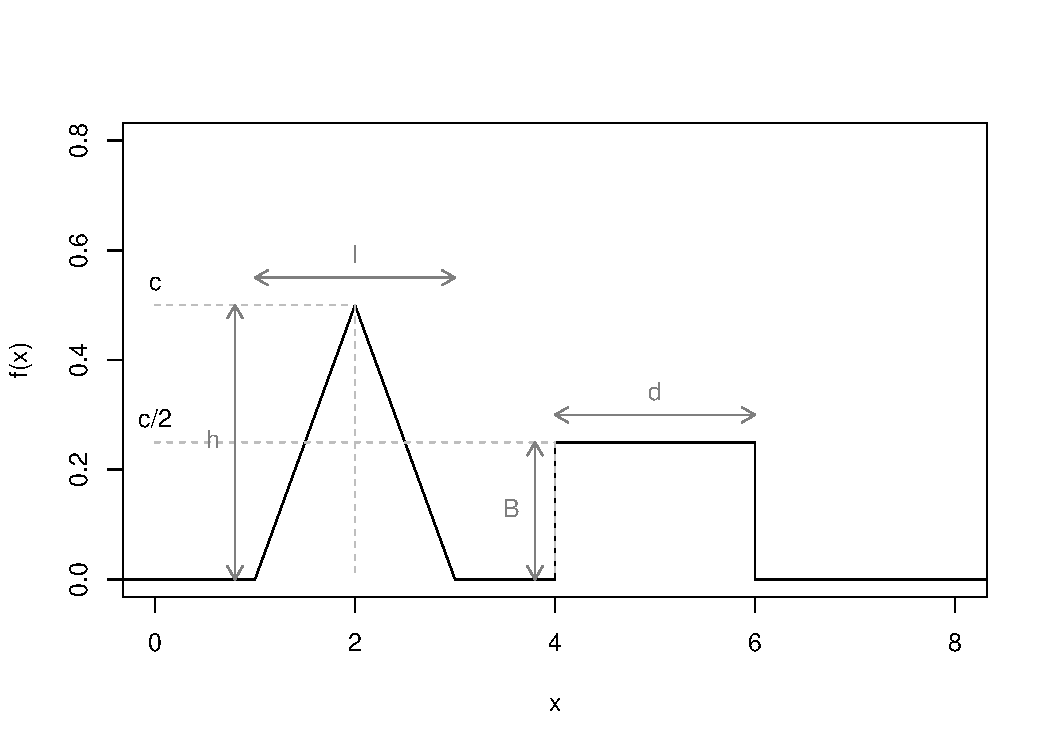
\includegraphics{figure_corrige.pdf}}

    \begin{center}
   \begin{description}
    \item[$l$]: length of the base of the triangle
    \item[$h$]: length of the height of the triangle
    \item[$d$]: length of the base of the rectangle
    \item[$B$]: length of the heightof the rectangle
    \end{description}
     \end{center}

    \newpage

\begin{enumerate}%[(a)]

  % ----------------------------------------- %

\item For $f(x)$ to be a density function, it is necessary that for all
$x$, $f(x) \ge 0$ and $\int_{-\infty}^{\infty}f(x)dx = 1$

  \begin{enumerate}[(a)]
  \item ) From the graphical representation we find that for all $x$ we have $f(x) \ge 0$. % est satisfait.
  \item To verify that $\int_{-\infty}^{\infty}f(x)dx = 1$  is satisfied, it is necessary to determine if there is a value $c$ so that the total area under the function $f(x)$ is equal to 1.


    \begin{eqnarray*}
      \int_{-\infty}^{\infty}f(x)dx  &=& \left. \text{triangle area} \ + \ \text{rectangle area} = \frac{lh}{2} + dB \right. \nonumber \\
       &=& \left. \frac{(3-1)c}{2} + (6-4)\frac{c}{2} = 2c \right. \nonumber
       \end{eqnarray*}

    Where we have that
       \begin{eqnarray*}
      \int_{-\infty}^{\infty}f(x)dx =1  &\iff& 2c =1.
    \end{eqnarray*}

    The only solution is $c = 0.5$.

  \end{enumerate}

  % ----------------------------------------- %

\item Graphically we find that the density function f (x) is a piecewise form function:

  \begin{equation*}
    f(x) = \left\{
      \begin{array}{ll}
        f_1(x) &\text{if } 1 < x \le 2 \\
        f_2(x) &\text{if } 2 < x \le 3 \\
        f_3(x) &\text{if } 4 < x \le 6 \\
        0  & \text{if not} \\
      \end{array}
    \right.
  \end{equation*}

  \begin{enumerate}[(a)]
  \item $f_1(x)$ is a line $a + bx$ found from the two points $(x_1, y_1) = (1,0)$ and $(x_2, y_2) =
    (2,0.5)$. We are looking for $a$ and $b$ such that  $f_{1}(x_{1}) = y_{1}$ and $f_{1}(x_{2}) = y_{2}$, i.e., we look for $a$ and $b$ such that $a+bx_{1}=y_{1}$ and $a+bx_{2}=y_{2}$. We find $a$ and $b$ with the equations:
    \begin{eqnarray*}
      b &=& \frac{y_2 - y_1}{x_2 - x_1} = \frac{0.5-0}{2-1} = 0.5 \\
      a &=& y_1 - b x_1 = 0 - 0.5 \cdot 1 = -0.5.
    \end{eqnarray*}
    So
    \begin{equation*}
      f_1(x) = -0.5 + 0.5x.
    \end{equation*}
  \item Similarly, $f_2(x)$ is a line $c + dx$ that we find from the two points $(x_2, y_2) = (2,0.5)$ and $(x_3,y_3) = (3,0)$:
    \begin{eqnarray*}
      d &=& \frac{y_3 - y_2}{x_3 - x_2} = \frac{0-0.5}{3-2} = -0.5 \\
      c &=& y_2 - b x_2 = 0.5 - (-0.5) \cdot 2 = 1.5.
    \end{eqnarray*}
    So
    \begin{equation*}
      f_2(x) = 1.5-0.5x.
    \end{equation*}
  \item And, finally,
    \begin{equation*}
      f_3(x) = \frac{c}{2} = \frac{0.5}{2} = 0.25.
    \end{equation*}
  \end{enumerate}

  % ----------------------------------------- %

\item The expectation of $X$ is defined as $\text{E}(X) = \int_{-\infty}^{\infty} x \cdot f(x) dx$.
  \begin{eqnarray*}
   \text{E}(X) &=& \int_{-\infty}^1 x \cdot 0 \ dx +
    \int_{1}^2 x \cdot f_{1}(x) \ dx +
    \int_{2}^3 x \cdot f_{2}(x) \ dx +
    \int_{3}^4 x \cdot 0 \ dx +
    \int_{4}^6 x \cdot f_{3}(x) \ dx\\
   && \quad +    \int_{6}^{+\infty} x \cdot 0 \ dx \\
    &=& \int_{1}^2 x \cdot (-0.5 + 0.5x) \ dx +
    \int_{2}^3 x \cdot (1.5-0.5x) \ dx +\int_{4}^6 x \cdot 0.25 \ dx \\
    &=& \int_{1}^{2} (-0.5x + 0.5x^2) \ dx +
    \int_{2}^{3} (1.5x - 0.5x^2) \ dx +
    \int_{4}^{6}0.25x \ dx \\
    &=& \left[ \frac{-0.5x^2}{2} + \frac{0.5x^3}{3} + c
    \right]^{2}_{1} +
    \left[ \frac{1.5x^2}{2} + \frac{-0.5x^3}{3} + c
    \right]^{3}_{2} +
    \left[ \frac{0.25x^2}{2} + c
    \right]^{6}_{4} \\
    &=& \left(\frac{-2}{2} + \frac{4}{3} - \frac{-0.5}{2}
      -\frac{0.5}{3} \right)
    + \left( \frac{13.5}{2} + \frac{-13.5}{3} - \frac{6}{2} +
      \frac{4}{3} \right)
    + \left( \frac{9}{2} - \frac{4}{2} \right) \\
    &=& {3.5}
  \end{eqnarray*}

  % ----------------------------------------- %

% \item La médiane est une valeur $m$ qui satisfait $F(m) = 0.5$. Dans notre cas, la surface du triangle est \'egale \`a la surface du rectangle (0.5). Ainsi la m\'ediane n'est pas unique car:
%
%   \begin{equation*}
%     F(x) = 0.5, \quad 3 < x \le 4.
%   \end{equation*}
%
%   Donc toutes les valeurs dans l'intervalle $]3, 4]$ satisfont la
%   d\'efinition de la m\'ediane. Si on veut une valeur unique, on peut
%   choisir le centre de l'intervalle, soit 3.5.

  % ----------------------------------------- %

\item Determine $P(X \ge 2)$, $P(X \le 4.5)$ and $P(2.5 \le X \le 5)$.

  \begin{enumerate}[(a)]
  \item $P(X \ge 2)$: Solution from the geometrical point of view:
    \begin{eqnarray*}
      P(X \ge 2) &=& 0.5 \text{ triangle area } + \text{ rectangle area } \\
      &=& 0.5 \cdot 0.5 + 0.5 \\ &=& {0.75}
    \end{eqnarray*}
Solution with density:
    \begin{eqnarray*}
      \int_2^3 (1.5-0.5x) \ dx + \int_4^6 0.25 \ dx &=& \left[ 1.5x - \frac{0.5x^2}{2} + c \right]^{3}_{2} + \left[ 0.25x  + c \right]^{6}_{4} \\
    &=&  0.25 + 0.5 = 0.75
    \end{eqnarray*}
    \item $P(X \le 4.5)$: Solution from the geometrical point of view:
    \begin{eqnarray*}
      P(X \le 4.5) &=& \text{ triangle area } + 0.25 \text{ rectangle area} \\
      &=& 0.5 + 0.25 \cdot 0.5 \\ &=& {0.625}
    \end{eqnarray*}
    Solution with density:
    \begin{eqnarray*}
    P(X \le 4.5) & = &  1-P(X>4.5) = 1- \int_{4.5}^6  0.25 \ dx \\
    & = & 1- \left[ 0.25x + c \right]^{6}_{4.5} = 1- 0.375 = 0.625
    \end{eqnarray*}

    \item $P(2.5 \le X < 5)$: Here it is necessary to integrate the first part $P(2.5 \le X < 3)$of the probability because the cut at 2.5 is placed in the middle of the lowering of the triangle.
    \begin{eqnarray*}
      P(2.5 \le X < 5) &=& \int_{2.5}^3 (1.5-0.5x) \ dx  + 0.5 \text{
        rectangle area} \\
      &=& \left[ 1.5x - \frac{0.5x^2}{2} + c \right]_{2.5}^3  +
      0.5 \cdot 0.5
      \\
      &=& 1.5 \cdot 3 - \frac{0.5 \cdot 3^2}{2} - 1.5 \cdot 2.5 +
      \frac{0.5 \cdot 2.5^2}{2} + 0.5 \cdot 0.5 \\
      &=& {0.3125}
    \end{eqnarray*}
  \end{enumerate}

\end{enumerate}

\bigskip

% ---------------------------------------------------------- %

\addtocounter{section}{1}
\section*{Exercise \thesection:}

Let $T$ be the random variable representing the waiting time of the bus, with $T \sim U(0,30)$. Its density function is therefore

\begin{equation*}
  f_T(t) = \left\{
    \begin{array}{ll}
      \frac{1}{30} & \text{if } 0 < t < 30 \\
      0 & \text{if not}
    \end{array}
  \right.
\end{equation*}
\medskip

\begin{enumerate}%[(a)]
\item The shape of the density implies that the distribution function is a piecewise function of form
  \begin{equation*}
    F_T(t) = \left\{
      \begin{array}{ll}
        0 & \text{if } t \le 0 \\
        F_{T,1}(t) & \text{if } 0 < t < 30 \\
        1 & \text{if } t \ge 30
      \end{array}
      \right.
  \end{equation*}
  By applying the definition $F(x)=P(X \le x)=\int_{-\infty}^x f(u)
  \ du$, we get $F_{T,1}(t)$ :
  \begin{equation*}
    F_{T,1}(t) =
    \int_{0}^{t} \frac{1}{30} du =
    \left[ \frac{u}{30} + c \right]^{t}_{0}
    = \frac{t}{30}.
  \end{equation*}
\item The probability of waiting more than 10 minutes is given by $P(T > 10)$, which can be calculated using the distribution function:
  \begin{equation*}
    P(T>10) = 1-P(T \le 10) = 1-F(10) = 1-\frac{10}{30} = \frac{2}{3}
    = {0.\bar{6}}.
  \end{equation*}
\item We search for the conditional probability
  $P(T>25 \ | \ T>15)$. So
  \begin{equation*}
    P(T>25 \ | \ T>15) = \frac{P(T>25 \ \cap \ T>15)}{P(T>15)} =
    \frac{P(T>25)}{P(T>15)} = \frac{1-P(T\le25)}{1-P(T\le15)} =
    \frac{1-25/30}{1-15/30} = \frac{1}{3} ={0.\bar{3}}.
  \end{equation*}
\end{enumerate}

\bigskip

% ---------------------------------------------------------- %

\addtocounter{section}{1}
\section*{Exercise \thesection:}

\begin{enumerate}%[(a)]
\item The random variable $Z$ takes values between 0 and 1, as $P( Z \le 1)=1$ so we have $F(1) = 1$. Thus:
  \begin{eqnarray*}
    F(1) = k \cdot \left( \frac{1}{3}-\frac{1}{2}+\frac{1}{5}\right) &=& 1 \\
    k \cdot \left( \frac{10-15+6}{30} \right)&=& 1% \\
    %  k &=& {30}
  \end{eqnarray*}
and so $k = {30}$.

  The density function $f(z)$ is the derivative of the distribution function, so
  \begin{eqnarray*}
    f(z) &=& F'(z) \\
    &=& 30\left(\frac{z^3}{3}-\frac{z^4}{2}+\frac{z^5}{5}\right)' \\
    &=& 30\left(\frac{3z^2}{3}-\frac{4z^3}{2}+\frac{5z^4}{5}\right) \\
    &=& 30\left(z^2 - 2z^3 + z^4\right)\\
    &=& {30z^2(1-z)^2} %\quad\quad 0 \le z \le 1
  \end{eqnarray*}
for $0 \le z \le 1$.

\item We calculate the expectation of $Z$ using the density found above:
  \begin{eqnarray*}
    \text{E}(Z) &=& \int_{0}^1 z \cdot f(z) \ dz \\
    &=& \int_0^1 z \cdot 30 (z^2 - 2z^3 + z^4) dz \\
    &=& 30 \int_{0}^1 (z^3 - 2z^4 + z^5) dz \\
    &=& 30 \left[ \frac{z^4}{4} - \frac{2z^5}{5} + \frac{z^6}{6} + c
      \right]^1_0  \\
    &=& 30 \left( \frac{1}{4} - \frac{2}{5} + \frac{1}{6} \right)
    = 30 \cdot \frac{25-24+10}{60} \\
    &=& {0.5}.
  \end{eqnarray*}

 The variance of $Z$ is given by the formula $\text{var}(Z) =
 \text{E}(Z^2) -\text{E}(Z)^2$.

We calculate first $\text{E}(Z^2)$:
  \begin{eqnarray*}
     \text{E}(Z^2) &=& \int_0^1 z^2 \cdot f(z) \ dz \\
    &=& \int_0^1 z^2 \cdot 30(z^2 - 2z^3 + z^4) \ dz \\
    &=& 30 \int_0^1 (z^4-2z^5+z^6) \ dz \\
    &=& 30 \left[ \frac{z^5}{5} + \frac{2z^6}{6} + \frac{z^7}{7} + c
      \right]_0^1  \\
    &=& 30 \cdot \frac{21-35+15}{105} = \frac{2}{7}.
  \end{eqnarray*}
  Then
  \begin{eqnarray*}
     \text{var}(Z) &=& \text{E}(Z^2)-\text{E}(Z)^2 \\
    &=& \frac{2}{7} - \left( \frac{1}{2} \right)^2 \\
    &=& \frac{8-7}{28} \approx {0.0357}.
  \end{eqnarray*}

\item We calculate $P(0.75 < Z < 1.5)$:
  \begin{eqnarray*}
    P(0.75 < Z < 1.5) &=& P(Z \le 1.5) -P(Z \le 0.75) \\
    &=& 1 - F(0.75) \\
    &=& 1 - 30 \cdot 0.75^3 \cdot \left( \frac{1}{3} - \frac{0.75}{2} +
      \frac{0.75^2}{5} \right) \\
    &\approx& {0.104};
  \end{eqnarray*}
   and $P(Z \ge 0.15)$:
   \begin{eqnarray*}
     P(Z \ge 0.15) &=& 1-P(Z < 0.15) \\
     &=& 1-F(0.15) \\
     &=& 1- 30 \cdot 0.15^3 \cdot \left( \frac{1}{3} - \frac{0.15}{2} +
      \frac{0.15^2}{5} \right) \\
    &\approx& {0.973}.
   \end{eqnarray*}
% \item Comme la moyenne est aussi égale à $0.5$, nous savons que la m\'ediane et la moyenne sont identiques. C'est une condition n\'ecessaire pour que la   distribution soit sym\'etrique.
%
% Remarque: la densit\'e est telle
%   que:
%   \begin{equation*}
%     f(z) = f(1-z), \forall z \in [0,1] \ \Longleftrightarrow \
%     f(0.5+x) = f(0.5-x), \forall x \in [-0.5,0.5]
%   \end{equation*}
%La distribution est donc bien sym\'etrique autour de 0.5.
%
%   \clearpage
 \item The probability that $Z$ is greater than 0.5 in the case $Z > 0.25$
  is given by
$$P ( Z \ge 0.5 \ | \ Z > 0.25).$$

We then calculate $P ( Z \ge 0.5 \ | \ Z > 0.25)$:
   \begin{eqnarray*}
     P ( Z \ge 0.5 \ | \ Z > 0.25) &=& \frac{P(Z \ge 0.5 \ \cap \ Z >
       0.25)}{P(Z > 0.25)} \\
     &=& \frac{P(Z \ge 0.5)}{P(Z > 0.25)} \\
     &=& \frac{1-P(Z<0.5)}{1-P(Z\le 0.25)} \\
     &=& \frac{1-F(0.5)}{1-F(0.25)} \\
     &=& \frac{1-30 \cdot 0.5^3 \left(\frac{1}{3}-\frac{0.5}{2} +
         \frac{0.5^2}{5}\right)}{1-30 \cdot 0.25^3 \left( \frac{1}{3} -
         \frac{0.25}{2} + \frac{0.25^2}{5}\right)} \\
     &\approx& {0.558}.
   \end{eqnarray*}
\end{enumerate}

\addtocounter{section}{1}
\section*{Exercise \thesection:}
%3.4 and 3.10

\begin{enumerate}
  \item The cumulative distribution of $X$ for  $x \geq 0$ is:
  \begin{equation*}
  F_X(x)= \int_0^x \lambda e^{-\lambda t} dt = -e^{-\lambda t} \bigg\vert_0^{x}= 1-e^{-\lambda x},
  \end{equation*}
  So:\begin{equation*}
  F_X(x) =
  \begin{cases}
   0                   & \text{if }  x < 0 \\
    1-e^{-\lambda x}      & \text{if } x \geq 0
  \end{cases}
  \end{equation*}
  \item The alpha quantile satisfies :
  \begin{eqnarray*}
    F(q_\alpha) &=& \alpha \\
    1-e^{-\lambda q_\alpha} &=& \alpha \\
    q_\alpha &=& \frac{\log(1-\alpha)}{-\lambda }
  \end{eqnarray*}
  \item First we should find $\lambda$ such that the $E(X)=8$.
\begin{equation*}
        E(X) = \int_0^\infty x \lambda e^{-\lambda x} dx
\end{equation*}
Integrating by part:
  \begin{eqnarray*}
    E(X) &=& -x e^{-\lambda x} \bigg\vert_0^{\infty} -\int_{0}^{\infty} -e^{-\lambda x} dx \\
     &=& -x e^{-\lambda x} \bigg\vert_0^{\infty} -    \frac{1}{\lambda} e^{-\lambda x} \bigg\vert_{0}^\infty \\
     &=& \frac{1}{\lambda}
  \end{eqnarray*}
 Then $E(X)=\frac{1}{\lambda}=8$ implies that $\lambda=\frac{1}{8}$.
 We can compute then the probability that lifetime of the television is more than 8 years:

 \begin{equation*}
    P(X>8)=1-P(X\leq 8)=1-(1-e^{-\frac{1}{8}8})=e^{-1}\simeq 0.37.
 \end{equation*}
 The median is $q_{\frac{1}{2}}$:
 \begin{equation*}
  q_{\frac{1}{2}} = \frac{\log(1-\frac{1}{2})}{-\lambda}=8\log(2) \simeq 5.54
 \end{equation*}
  \item Let's first compute $E(X^2)$:
  \begin{eqnarray*}
  E(X^2)&=& \int_{0}^{\infty} \frac{x^2}{8} e^{-\frac{x}{8}} dx = -x^2 e^{\frac{-x}{8}} \bigg\vert_{0}^{\infty} - \int_{0}^{\infty} -2x e^{\frac{-x}{8}}dx  \\
  &=& -x^2 e^{\frac{-x}{8}} \bigg\vert_{0}^{\infty} + 2\cdot 8 \int_{0}^{\infty} \frac{x}{8} e^{\frac{-x}{8}}dx=0 +2 \cdot 8 E(X) \\
  &=& 2\cdot 8^2=128
  \end{eqnarray*}
  Then we can compute the variance:
  \begin{equation*}
    Var(X)=E(X^2)-E(X)^2=128-8^2=64=E(X)^2
  \end{equation*}
\end{enumerate}


\addtocounter{section}{1}
\section*{Exercise \thesection:}

% ex 3.7

\begin{enumerate}
  \item To determine $C$ and $\lambda$ we will use:
  \begin{eqnarray*}
  % \nonumber to remove numbering (before each equation)
    \int_0^{\infty} C v \exp(-\lambda v)dv&=& 1 \\
    \text{and} \qquad E(V) &=& \int_0^{\infty} C v^2 \exp(-\lambda v)dv = 30.
  \end{eqnarray*}

\begin{enumerate}
  \item Let's integrate by part:
  \begin{eqnarray*}
    \int_0^{\infty} C v \exp(-\lambda v)dv &=& \frac{-1}{\lambda} Cv \exp(-\lambda v)\bigg\vert_0^\infty + C \int_0^\infty \frac{1}{\lambda} \exp(-\lambda v) dv\\
     &=&  0- \frac{C}{\lambda^2}  \exp(-\lambda v) \bigg\vert_0^\infty = \frac{C}{\lambda^2} =1  \Leftrightarrow C=\lambda^2
  \end{eqnarray*}

  \item
    \begin{eqnarray*}
    C \int_0^{\infty}  v^2 \exp(-\lambda v)dv &=& \frac{-1}{\lambda} Cv^2 \exp(-\lambda v)\bigg\vert_0^\infty + C \int_0^\infty \frac{1}{\lambda} 2v\exp(-\lambda v) dv\\
     &=&  \frac{2}{\lambda} \int_0^\infty C v\exp(-\lambda v) dv = \frac{2}{\lambda}= 30  \\
     \Leftrightarrow \lambda &=& \frac{1}{15}  \Rightarrow C=\frac{1}{225}
  \end{eqnarray*}
\end{enumerate}


  \item Let $T=\frac{15}{V}$. It's cumulative distribution function is:
  \begin{equation*}
  F_T(t)=P(T<t)=P\left(\frac{15}{V}<t\right)=P\left(V>\frac{15}{t}\right)=1-F_V\left(\frac{15}{t}\right).
  \end{equation*}
  We deduce its density:
  \begin{equation*}
  f_T(t)=\frac{15}{t^2}f_V\left(\frac{15}{t}\right)=\frac{1}{t^3} \exp\left(-\frac{1}{t}\right).
  \end{equation*}

  Finally we can compute the expectation of $T$:
  \begin{eqnarray*}
    E(T) &=& \int_0^\infty t \frac{1}{t^3} \exp\left(-\frac{1}{t}\right) dt \\
     &=& \exp\left(-\frac{1}{t}\right) \bigg\vert_{t=0}^{t=\infty}=1
  \end{eqnarray*}
\end{enumerate}



\end{document}



